\documentclass{beamer}
\usepackage{geometry}
\usepackage[english]{babel}
\usepackage[utf8]{inputenc}
\usepackage{amsmath}
\usepackage{amsfonts}
\usepackage{amssymb}
\usepackage{tikz}
\usetikzlibrary{quotes, angles}
\usepackage{graphicx}

%\usepackage{pgfplots}
%\pgfplotsset{width=10cm,compat=1.9}
%\usepackage{pgfplotstable}

\setlength{\headheight}{26pt}%doesn't seem to fix warning

\usepackage{fancyhdr}
\pagestyle{fancy}
\fancyhf{}

%\rhead{\small{4 March 2019}}
\lhead{\small{BECA / Dr. Huson / Geometry - Unit 8 Transformational Geometry}}

\renewcommand{\headrulewidth}{0pt}

\title{10th Grade Geometry - Unit 8: Transformational Geometry}
\subtitle{Bronx Early College Academy}
\author{Christopher J. Huson PhD}
\date{4 March 2019}

\begin{document}
\frame{\titlepage}
\section[Outline]{}
\frame{\tableofcontents}


\section{Laptops - Geogebra class codes}
  \frame
  {
    \frametitle{GQ: How do we model with digital tools?}
    \framesubtitle{CCSS: HSG.CO.D.12 Congruence, geometric constructions \hspace{\stretch{1}} \alert{7.1 Tuesday 18 January}}

    GeoGebra Geometry App\\
    Enter \alert{N7BHK} for 10.1 or \alert{P9PNZ} for 10.2\\
    Set up account using your real name.\\
    Beginner Tutorials with Lesson Ideas\\
    Author: Tim Brzezinski\\[0.5cm]
    Homework: Complete Geogebra
  }

\section{8.1 Geogebra - Transformations project Tuesday 6 March}
  \frame
  {
    \frametitle{GQ: How do we use technology to explore geometric relationships?}
    \framesubtitle{CCSS: MP5 Use appropriate tools strategically: dynamic geometry software \hfill \alert{8.1 Tuesday 6 March}}

    \begin{block}{Lesson: Geogebra project showing various transformations}
      \begin{enumerate}
        \item Apply transformations to polygons (show at least two)
        \item Use Geogebra's formating tools
        \item Label with the transformation's specifics (e.g. center, factor)
        \item Rubric: correct, aesthetics, \alert{MLA \& email standards}
        \item Export a .png to email me. (husonbeca@gmail.com)
        \item Filename: Last-Title.png, email subject line message
      \end{enumerate}
    \end{block}
    \alert{Parent conferences this Thursday evening, Friday afternoon}\\
    Homework: Test corrections  (due tomorrow)
  }

\section{8.2 Dilation and similar triangles. Wednesday 7 March}
  \frame
  {
    \frametitle{GQ: How do we transform objects on the coordinate plane?}
    \framesubtitle{CCSS: HSG.CO.D.12 Congruence, geometric constructions \hfill \alert{8.2 Wednesday 7 March}}

    \begin{block}{Do Now Plotting transformations review review}
      \begin{enumerate}
        \item Handout
      \end{enumerate}
    \end{block}
    Lesson: Translation, reflection, rotation, dilation, composition, properties\\[0.5cm]
    Homework: Practice problems handout
  }

\section{8.3 Dilation and similar triangles. Thursday 8 March}
  \frame
  {
    \frametitle{GQ: How do we transform objects on the coordinate plane?}
    \framesubtitle{CCSS: HSG.CO.D.12 Congruence, geometric constructions \hfill \alert{8.3 Thursday 8 March}}

    \begin{block}{Do Now Analytic geometry review}
      \begin{enumerate}
        \item Point-slope form of linear equations
        \item Applications of slope, graphing linear equations
        \item The equation of a circle, deriving center and radius
      \end{enumerate}
    \end{block}
    Lesson: Midlines, medians, the centroid. Measuring with Geogebra, submissions standards\\[0.5cm]
    Homework: Practice problems handout
  }

\section{8.4 Symmetry, "onto" transformations. Monday 11 March}
  \frame
  {
    \frametitle{GQ: How do we say that objects are mapped "onto" themselves?}
    \framesubtitle{CCSS: HSG.CO.D.12 Congruence, geometric constructions \hfill \alert{8.4 Monday 11 March}}

    \begin{block}{Do Now Analytic geometry practice}
      \begin{enumerate}
        \item Point-slope form of linear equations
        \item Applications of slope, graphing linear equations
        \item The equation of a circle, deriving center and radius
      \end{enumerate}
    \end{block}
    Lesson: SSS Similarity;
    \\Symmetry in terms of tranformations \emph{onto} oneself\\[0.5cm]
    Homework: Practice problems handout
  }

\section{8.5 Geogebra - Reflected+dilated $\triangle$ similarity Tues 12 March}
  \frame
  {
    \frametitle{GQ: How do we use technology to explore geometry?}
    \framesubtitle{CCSS: MP5 Use appropriate tools strategically: dynamic geometry software \hfill \alert{8.5 Tuesday 12 March}}

    \begin{block}{Lesson: Combining Geogebra and Microsoft Word}
      \begin{enumerate}
        \item Reflect $\triangle ABC$ across the bisector of $\angle A$, yielding $\triangle A'B'C'$
        \item Dilate $\triangle A'B'C' \rightarrow \triangle A''B''C''$ ($\triangle A'B'C'$ is then hidden)
        \item Spicy: measure corresponding sides and/or angles
        \item Export a .png file. Insert it in Word, adding heading \& title.
        \item Spicy: add text and formulas using Microsoft's formula bar
        \item Email me: Last-Title.pdf, with subject line \& message
        \item Rubric: correct, aesthetics, MLA \& email standards
      \end{enumerate}
    \end{block}
    \alert{$\pi$ Day, Friday afternoon}\\
    Homework: Complete project (due by 10:00 pm)
  }

\section{8.5 Geogebra construction}
  \frame
  {
    \frametitle{The red triangle has been reflected across its angle bisector and dilated from its own vertex}
    \framesubtitle{Hide the intermediate triangle so only the preimage and final image are shown.}

    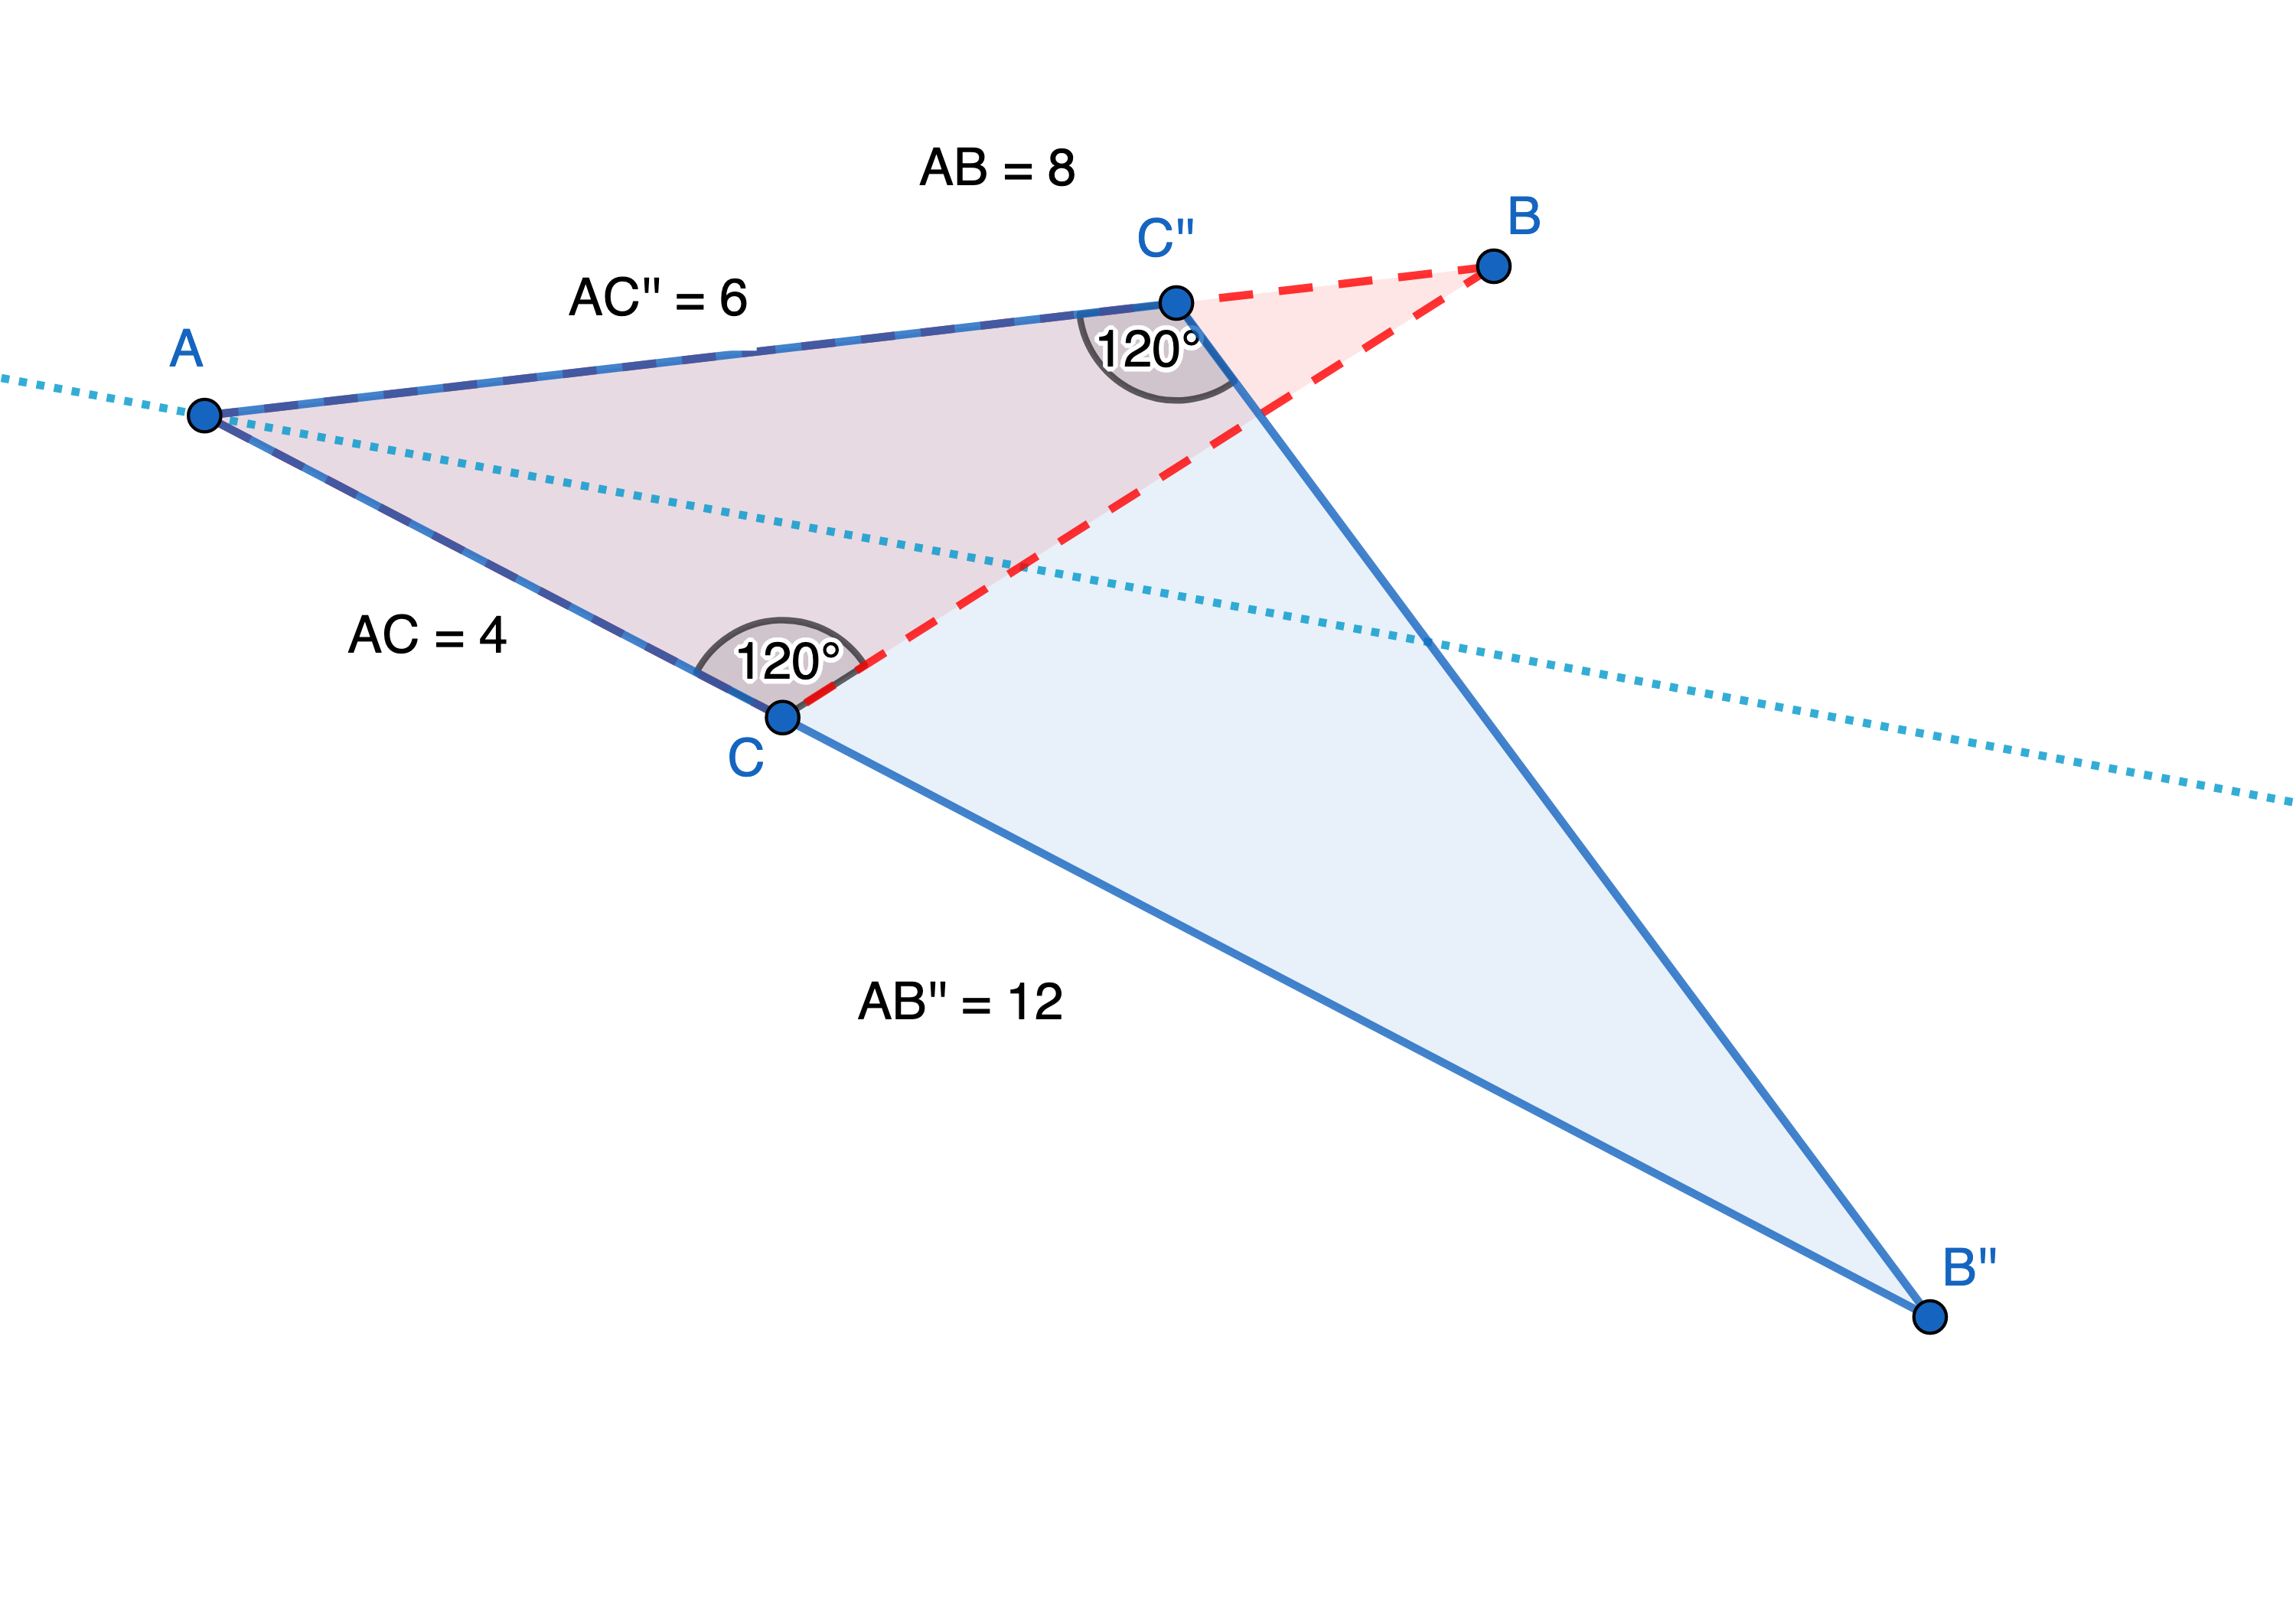
\includegraphics[width=0.8\textwidth]{8-6Similar-Triangle-Reflection.png}

    The Geogebra image file should be inserted into Microsoft Word\\
    Spicy: angle measures and segment lengths
  }

\section{8.5 Geogebra - Secant segment length relationships}
  \frame
  {
    \frametitle{Two circle secants form two similar (reflected) triangles}
    %\framesubtitle{Hide the intermediate triangle so only the preimage and final image are shown.}

    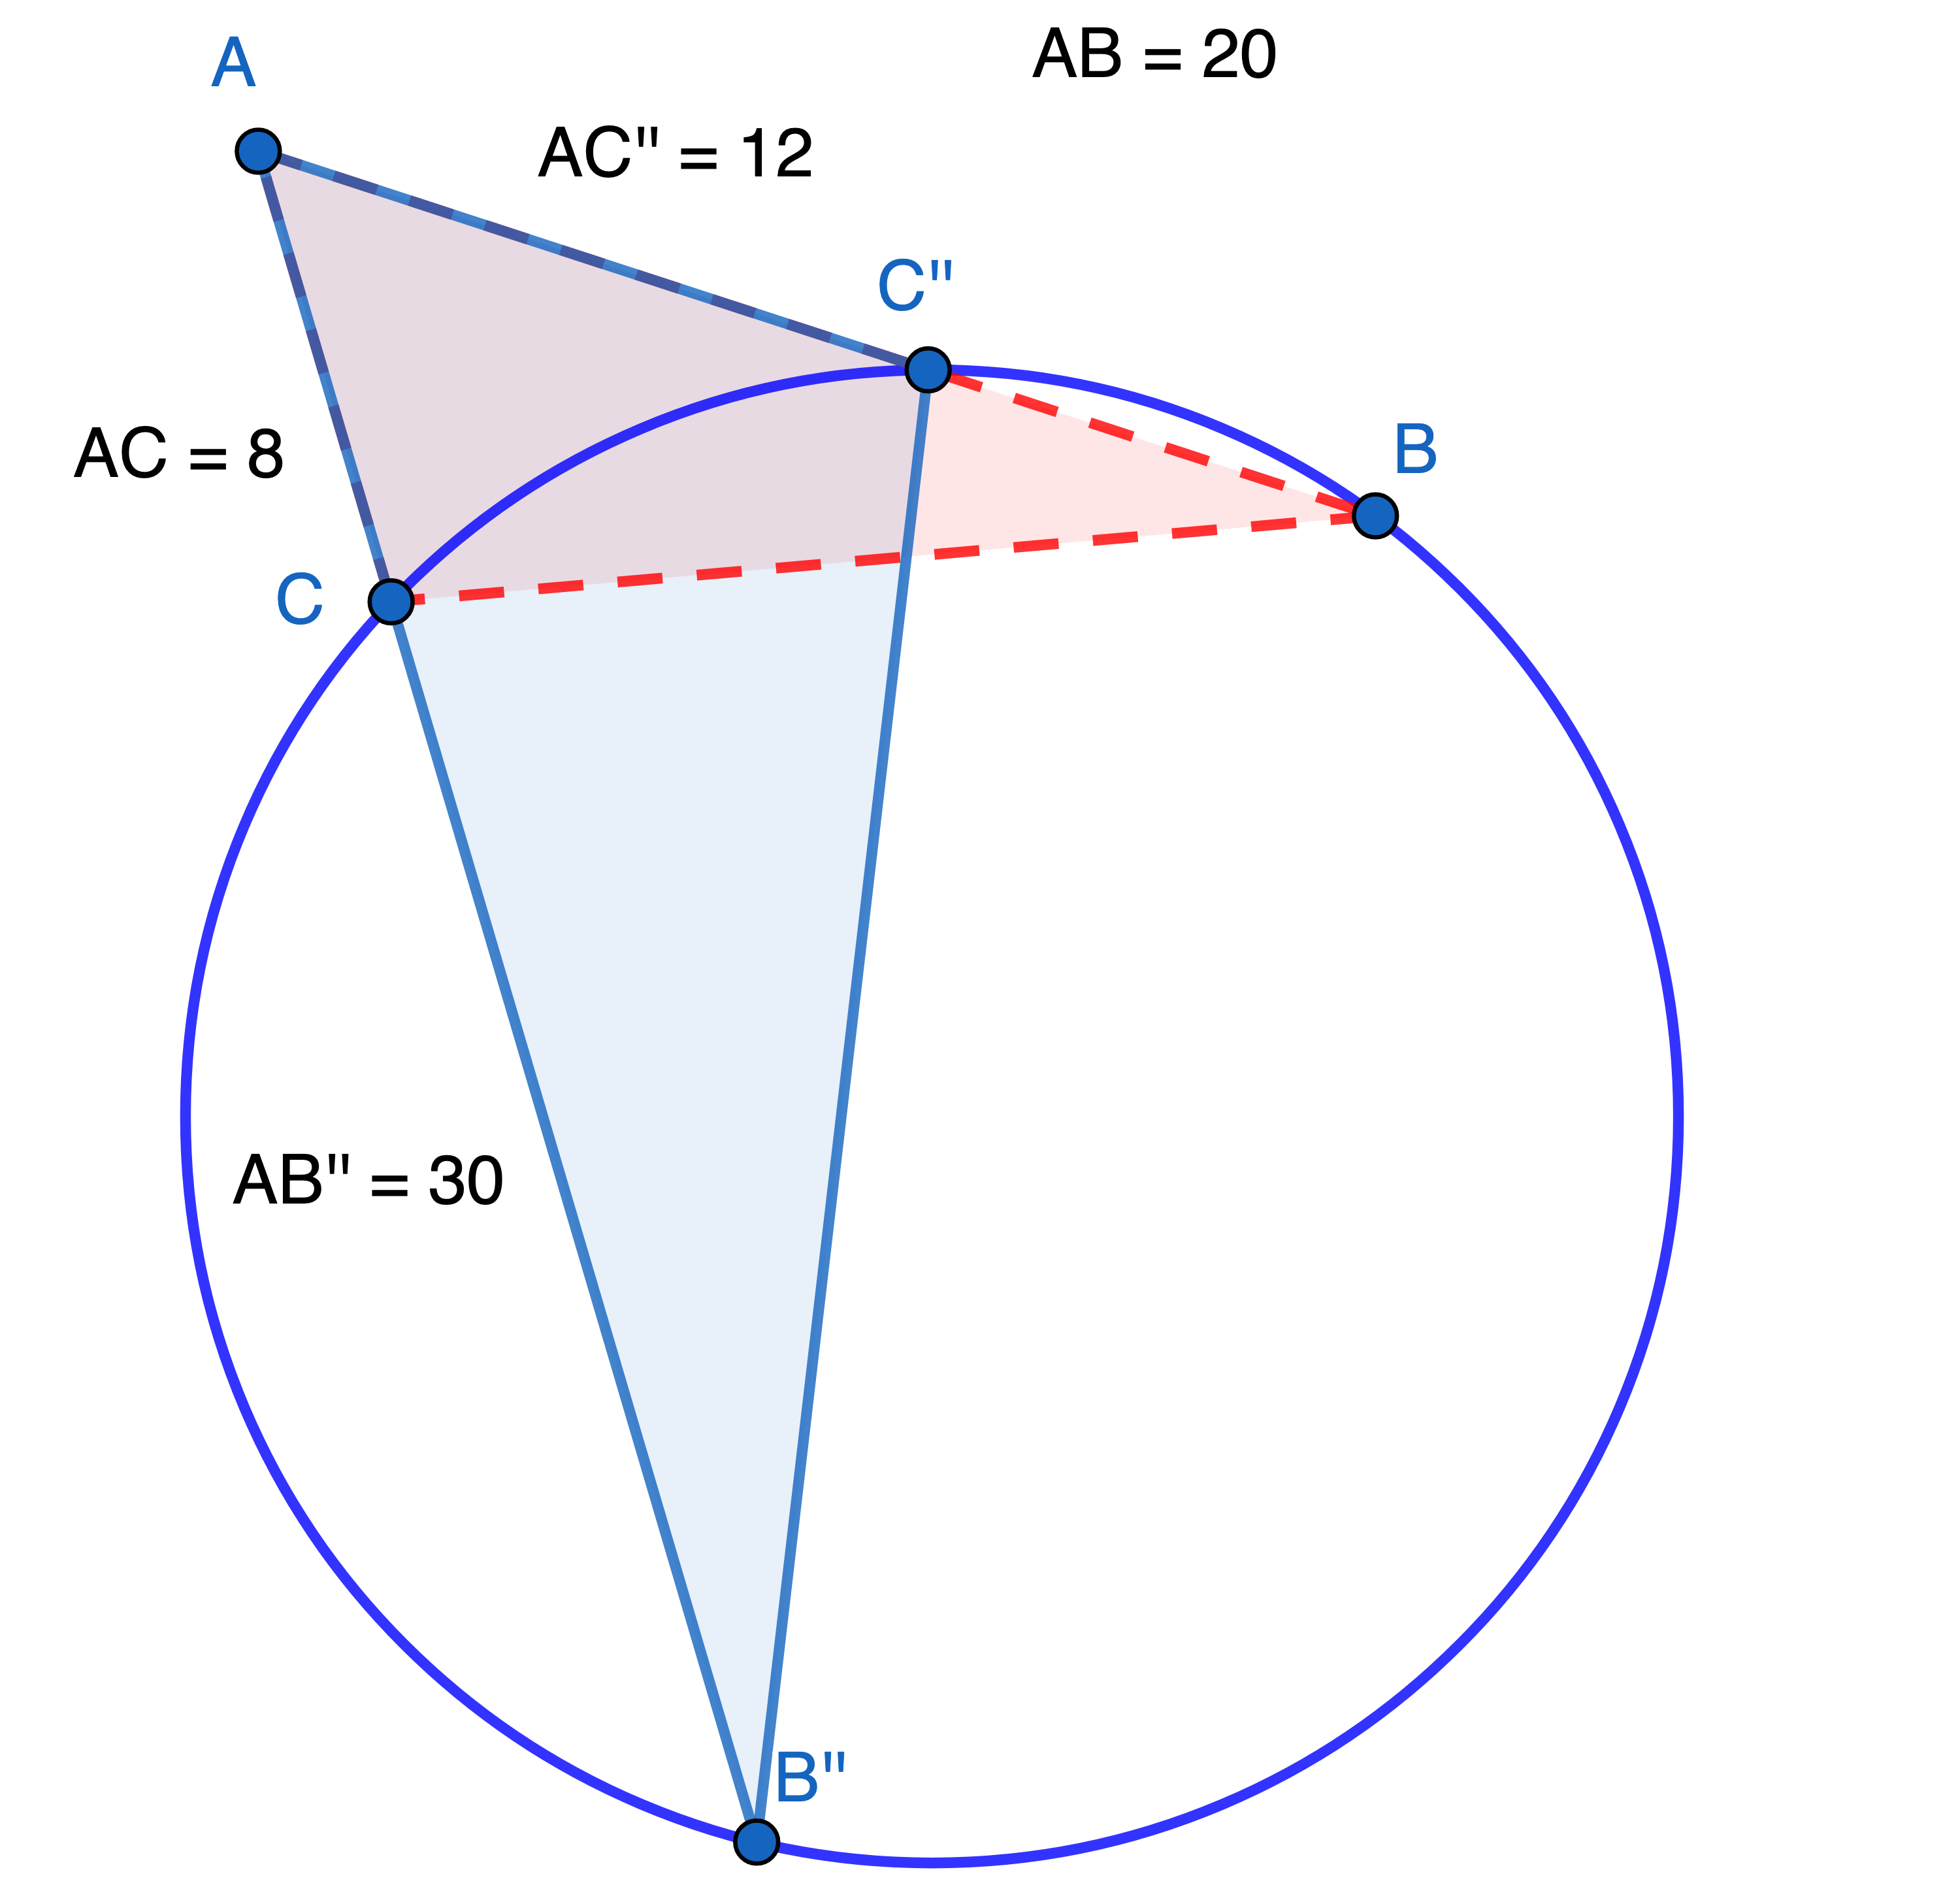
\includegraphics[width=0.7\textwidth]{8-6Similar-Triangle-Circle.png}
  }

\section{8.7 SAS Similarity: secants. Wednesday 13 March}
  \frame
  {
    \frametitle{GQ: How do we use the scale factor to calculate segment lengths?}
    \framesubtitle{CCSS: HSG.CO.D.12 Congruence, geometric constructions \hfill \alert{8.7 Wednesday 13 March}}

    \begin{block}{Do Now Similar triangle handout}
      \begin{enumerate}
        \item Naming corresponding relationships
        \item Determining equal ratios (to scale factor)
        \item Applying similarity relationships in situations
      \end{enumerate}
    \end{block}
    Lesson: SAS Similarity;
    \\Rotational symmetry\\[0.5cm]
    Homework: Practice problems handout
  }

\section{8.8 Rotational symmetry. Thursday 14 March}
  \frame
  {
    \frametitle{GQ: How do we calculate angles of rotation mapping "onto" itself?}
    \framesubtitle{CCSS: HSG.CO.D.12 Congruence, geometric constructions \hfill \alert{8.8 Thursday 14 March}}

    \begin{block}{Do Now Similar triangle handout}
      \begin{enumerate}
        \item Naming corresponding relationships
        \item Determining equal ratios (to scale factor)
        \item Applying similarity relationships in situations
      \end{enumerate}
    \end{block}
    Lesson: SAS Similarity;
    \\Rotational symmetry\\[0.5cm]
    Homework: Practice problems handout
  }

\section{8.9 Similarity practice Friday 15 March}
  \frame
  {
    \frametitle{GQ: How do we use the scale factor to calculate segment lengths?}
    \framesubtitle{CCSS: HSG.CO.D.12 Congruence, geometric constructions \hfill \alert{8.9 Friday 15 March}}

    \begin{block}{Do Now Similar triangle handout}
      \begin{enumerate}
        \item Naming corresponding relationships
        \item Determining equal ratios (to scale factor)
        \item Applying similarity relationships in situations
      \end{enumerate}
    \end{block}
    Lesson: Common situations with similar triangles\\
    Assessment: pop quiz\\[0.5cm]
    Homework: Practice problems handout
  }

\section{8.10 Project conventions/requirements Monday 18 March}
  \frame
  {
    \frametitle{GQ: How do we use the scale factor to calculate segment lengths?}
    \framesubtitle{CCSS: HSG.CO.D.12 Congruence, geometric constructions \hfill \alert{8.10 Monday 18 March}}

    \begin{block}{Do Now Similar triangle handout}
      \begin{enumerate}
        \item Naming corresponding relationships
        \item Determining equal ratios (to scale factor)
        \item Applying similarity relationships in situations
      \end{enumerate}
    \end{block}
    Lesson: Common situations with similar triangles, chords\\
    Assessment: Project requirements\\[0.5cm]
    Homework: Practice problems handout
  }

\section{8.11 Geogebra - Common $\triangle$ dilation situations Tuesday 19 March}
  \frame
  {
    \frametitle{GQ: How do we use technology to explore geometry?}
    \framesubtitle{CCSS: MP5 Use appropriate tools strategically: dynamic geometry software \hfill \alert{8.11 Tuesday 19 March}}

    \begin{block}{Project: Common Triangle Dilation Situations}
      \begin{enumerate}
        \item Write a paper diagramming common similar triangle examples
        \item Spicy: Use color \& line variations for clarity (not decoration)
        \item Construct in Geogebra, compile in Word: add heading \& title, text, and formulas using Microsoft's equation editor
        \item Email me: Last-Title.pdf, with subject line \& message
        \item Rubric: correct, aesthetics, MLA \& email standards
      \end{enumerate}
    \end{block}
    \alert{Unit test Thursday}\\
    Homework: Complete project (due by 10:00 pm), problem set
  }

\section{8.12 Review for unit test Wednesday 20 March}
  \frame
  {
    \frametitle{GQ: How do we use the scale factor to calculate segment lengths?}
    \framesubtitle{CCSS: HSG.CO.D.12 Congruence, geometric constructions \hfill \alert{8.12 Wednesday 20 March}}

    \begin{block}{Do Now Similar triangle handout}
      \begin{enumerate}
        \item Naming corresponding relationships
        \item Determining equal ratios (to scale factor)
        \item Applying similarity relationships in situations
      \end{enumerate}
    \end{block}
    Lesson: Common situations with similar triangles\\
    Assessment: \alert{Unit test tomorrow}\\[0.5cm]
    Homework: Study for test
  }

\section{8.13 Unit test Thursday 21 March}
  \frame
  {
    \frametitle{GQ: How do we use the scale factor to calculate segment lengths?}
    \framesubtitle{CCSS: HSG.CO.D.12 Congruence, geometric constructions \hfill \alert{8.13 Thursday 21 March}}


    Assessment: \alert{Unit test}\\[0.5cm]
    Homework: Practice problems handout
  }


\end{document}
